\documentclass[11pt]{beamer}

\usetheme{Madrid}

\usepackage[french]{babel}
\usepackage{amsmath, amssymb, amsfonts}
\usepackage{graphicx}

\title{Adaptation de domaine et bornes théoriques}
\author{Jean Constantin GEORGES}
\institute{Université d'Angers}
\date{19 Juin 2026}

\begin{document}

%------------------------------------------------
\begin{frame}
    \titlepage
\end{frame}
%------------------------------------------------


%------------------------------------------------


%------------------------------------------------
\begin{frame}{Motivation}

En apprentissage supervisé classique, on suppose que :

\[
D_{\text{train}} = D_{\text{test}}
\]

\vspace{0.3cm}

En pratique, cette hypothèse est souvent fausse :

\begin{itemize}
    \item images synthétiques vs images réelles ;
    \item données médicales provenant d’hôpitaux différents ;
    \item reconnaissance vocale avec accents différents.
\end{itemize}

\vspace{0.3cm}

\textbf{Question :}

Peut-on transférer un modèle appris sur un domaine source vers un domaine cible différent ?

\end{frame}
%------------------------------------------------




\begin{frame}{Cadre de l’adaptation de domaine}

\textbf{Définition d’un domaine}

\vspace{0.3cm}

Un domaine est défini par une paire :
\[
\langle D, f \rangle
\]

où :
\begin{itemize}
    \item $D$ est une distribution de probabilité sur l’espace d’entrée $X$ ;
    
    \item $f : X \rightarrow [0,1]$ est une fonction d’étiquetage.
\end{itemize}

\vspace{0.3cm}

Dans ce travail :
\[
f(x) = \mathbb{P}(Y=1 \mid X=x)
\]

avec $Y \in \{0,1\}$.

\vspace{0.3cm}

Nous considérons deux domaines :
\[
\langle D_S, f_S \rangle
\qquad \text{et} \qquad
\langle D_T, f_T \rangle
\]

\end{frame}




\begin{frame}{Hypothèses et erreurs}

\textbf{Hypothèse de classification}

\vspace{0.2cm}

Une hypothèse est une fonction : $
h : X \rightarrow \{0,1\}$

qui prédit une classe à partir d’une donnée d’entrée $x$.

\vspace{0.3cm}

\textbf{Erreur sur le domaine source}
\[
\varepsilon_S(h,f_S)
=
\mathbb{E}_{x \sim D_S}
\left[
|h(x)-f_S(x)|
\right]
\]

Lorsque la fonction d’étiquetage est implicite :  $
\varepsilon_S(h)
=
\varepsilon_S(h,f_S)$

\vspace{0.3cm}

\textbf{Erreur sur le domaine cible} :  $
\varepsilon_T(h)
=
\varepsilon_T(h,f_T)$

\vspace{0.4cm}

\textbf{Objectif}

Trouver une hypothèse $h$ minimisant l’erreur cible tout en utilisant principalement des données du domaine source.

\end{frame}



\begin{frame}{Rôle de la divergence entre distributions}

\textbf{Comparer les domaines source et cible}

\vspace{0.3cm}

Une mesure naturelle de différence entre distributions est la
distance de variation totale :
\[
d_1(D,D')
=
2
\sup_{B \in \mathcal{B}}
\left|
\Pr_D(B)-\Pr_{D'}(B)
\right|
\]

\vspace{0.2cm}

où $\mathcal{B}$ désigne l’ensemble des parties mesurables.


\vspace{0.2cm}

\textbf{Interprétation}

\begin{itemize}
    \item $d_1$ mesure la différence maximale entre deux distributions ;
    
    \item si $d_1$ est grand, les domaines sont très différents ;
    \item si $d_1$ est petit, les domaines sont proches.
\end{itemize}

\end{frame}



\begin{frame}{La H-divergence}

La H-divergence mesure la capacité d’une classe
d’hypothèses à distinguer deux distributions.

\vspace{0.2cm}

\textbf{Définition}

Soit $H$ une classe d’hypothèses sur $X$.

Pour toute hypothèse $h \in H$, on définit :
\[
I(h)=\{x \in X \mid h(x)=1\}
\]

La H-divergence entre $D$ et $D'$ est :

\[
d_H(D,D')
=
2
\sup_{h \in H}
\left|
\Pr_D(I(h))
-
\Pr_{D'}(I(h))
\right|
\]

\vspace{0.2cm}

\textbf{Interprétation} : 
Même interpretation avec $d_1$

\vspace{0.3cm}

On peut affirmer que : 
\[
d_H(D,D')
\leq
d_1(D,D')
\]

\end{frame}


\begin{frame}{Première borne entre erreur source et erreur cible}

\textbf{Théorème 1} : Liaison entre erreurs source et cible

\vspace{0.2cm}

Pour toute hypothèse $h \in H$ :
\[
\varepsilon_T(h)
\leq
\varepsilon_S(h)
+
d_1(D_S,D_T)
+
\min
\left\{
\mathbb{E}_{D_S}[|f_S(x)-f_T(x)|],
\mathbb{E}_{D_T}[|f_S(x)-f_T(x)|]
\right\}
\]

\vspace{0.4cm}

\textbf{Interprétation}

\begin{itemize}
    
    \item $|f_S-f_T|$ :
    mesure si les deux domaines sont d'accord sur son étiquette
\end{itemize}

\vspace{0.4cm}

\textbf{Conséquence}

Une faible erreur source ne suffit pas :
les distributions et les fonctions d’étiquetage
doivent aussi être proches.

\end{frame}



\begin{frame}{Idée de la preuve du Théorème 1}

On part de : $
\varepsilon_T(h)=\varepsilon_T(h,f_T)$ \\

et on ajoute puis soustrait des termes intermédiaires :

\[
\varepsilon_S(h,f_S)
\qquad \text{et} \qquad
\varepsilon_S(h,f_T)
\]

\vspace{0.1cm}

Après réorganisation :
\[
\varepsilon_T(h)
\leq
\varepsilon_S(h)
+
|\varepsilon_S(h,f_T)-\varepsilon_S(h,f_S)|
+
|\varepsilon_T(h,f_T)-\varepsilon_S(h,f_T)|
\]

\vspace{0.1cm}

\textbf{Contrôle des deux termes}
\[
|\varepsilon_S(h,f_T)-\varepsilon_S(h,f_S)|
\leq
\mathbb{E}_{D_S}[|f_S(x)-f_T(x)|]
\]

\[
|\varepsilon_T(h,f_T)-\varepsilon_S(h,f_T)|
\leq
d_1(D_S,D_T)
\]
\vspace{0.1cm}

On obtient finalement la borne du théorème.

\end{frame}



\begin{frame}{Estimation empirique de la H-divergence}

\textbf{Lemme 4.1}

\vspace{0.1cm}
Soit $\mathcal{H}$ une classe d’hypothèses définie sur $X$, de dimension VC $d$. \\
Soient $U$ et $U'$ deux échantillons de taille $m$, tirés respectivement selon les distributions $D$ et $D'$. \\
Soit $\hat{d}_{\mathcal{H}}(U, U')$ la H-divergence empirique calculée à partir de ces échantillons.

\vspace{0.2cm}

Alors, avec probabilité au moins $1-\delta$ :
\[
d_H(D,D')
\leq
\hat d_H(U,U')
+
4
\sqrt{
\frac{
d\log(2m)+\log\left(\frac{2}{\delta}\right)
}{m}
}
\]

\vspace{0.2cm}

\textbf{Interprétation}

\begin{itemize}
    \item la H-divergence peut être estimée à partir d’échantillons finis ;
    
    \item plus $m$ augmente,
    plus l’estimation empirique devient précise.
\end{itemize}

\end{frame}






\begin{frame}{Lemme 4.2 : interprétation de la H-divergence}

\textbf{Lemme 4.2}

\vspace{0.3cm}

Soit $H$ une classe d’hypothèses symétrique.

Alors :

\[
\hat d_H(U,U')
=
2
\left(
1-
\min_{h \in H}
\left[
\frac{1}{m}
\sum_{x:h(x)=0}\mathbf{1}_{x\in U}
+
\frac{1}{m}
\sum_{x:h(x)=1}\mathbf{1}_{x\in U'}
\right]
\right)
\]

\vspace{0.3cm}

\textbf{Interprétation}

\vspace{0.2cm}

\begin{itemize}
    \item les données source reçoivent le label $0$ ;
    
    \item les données cible reçoivent le label $1$ ;
    
    \item on cherche l’hypothèse séparant le mieux les deux domaines.
\end{itemize}

\vspace{0.3cm}

La H-divergence mesure donc la capacité
d’un classificateur à distinguer
les distributions source et cible.

\end{frame}




\begin{frame}{Hypothèse idéale et espace $H\Delta H$}

\textbf{Hypothèse jointe idéale}
\vspace{0.1cm}
\[
h^*
=
\arg\min_{h \in H}
\left(
\varepsilon_S(h)+\varepsilon_T(h)
\right)
\]

\vspace{0.1cm}

On définit : $
\lambda
=
\varepsilon_S(h^*)
+
\varepsilon_T(h^*)$

\vspace{0.1cm}

\textbf{Interprétation de $\lambda$}

\begin{itemize}
    \item si $\lambda$ est faible :
    une hypothèse performante existe sur les deux domaines ;
    
    \item si $\lambda$ est grand :
    l’adaptation devient difficile voire impossible.
\end{itemize}

\vspace{0.4cm}

\textbf{Espace de différence symétrique}

\[
g \in H\Delta H
\iff
g(x)=h(x)\oplus h'(x)
\]

avec $h,h' \in H$ et $\oplus$ désigne l’opérateur XOR.

\vspace{0.2cm}

L'espace $H\Delta H$ permet de définir une divergence plus fine entre distributions appelée $H\Delta H$-divergence.

\end{frame}



\begin{frame}{Lemme 4.3 — Contrôle de la différence d’erreur}

\textbf{Lemme 4.3.} Pour toutes hypothèses $h,h' \in \mathcal H$ :

\[
\left|
\varepsilon_S(h,h')
-
\varepsilon_T(h,h')
\right|
\le
\frac12 d_{\mathcal H \Delta \mathcal H}(D_S,D_T).
\]

\vspace{0.2cm}

Avec : 
\[
d_{\mathcal{H}\Delta\mathcal{H}}(D_S, D_T)
= 2 \sup_{h, h' \in \mathcal{H}}
\left| \Pr_{x \sim D_S}\bigl[h(x) \neq h'(x)\bigr]
- \Pr_{x \sim D_T}\bigl[h(x) \neq h'(x)\bigr] \right|.
\]

\vspace{0.2cm}

\textbf{Interprétation :}

\begin{itemize}
    \item Le lemme compare le désaccord entre deux hypothèses
    sur les domaines source et cible.
    
    \item Si la divergence 
    $d_{\mathcal H \Delta \mathcal H}(D_S,D_T)$
    est faible : $
    \varepsilon_S(h,h')
    \approx
    \varepsilon_T(h,h')$
    
    \item Donc les comportements des hypothèses restent similaires
    sur les deux domaines.
\end{itemize}

\vspace{0.3cm}

\textbf{Idée clé :}
$\mathcal H \Delta \mathcal H$
mesure uniquement les régions où les hypothèses de $\mathcal H$
se contredisent.

\end{frame}






\begin{frame}{Théorème 2 — Borne fondamentale}

\textbf{Théorème 2.}  
Soit $\mathcal H$ une classe d’hypothèses de dimension VC $d$.

\vspace{0.2cm}

Pour toute hypothèse $h \in \mathcal H$, avec probabilité au moins
$1-\delta$ :
\[
\varepsilon_T(h)
\le
\varepsilon_S(h)
+
\frac12
\hat d_{\mathcal H \Delta \mathcal H}(U_S,U_T)
+
4
\sqrt{
\frac{
2d\log(2m')
+
\log\left(\frac{2}{\delta}\right)
}{m'}
}
+
\lambda.
\]

\vspace{0.3cm}

\textbf{Idée générale :}

La performance sur le domaine cible dépend :
\begin{itemize}
    \item de la performance sur le domaine source ;
    \item de la différence entre les distributions ;
    \item de l’existence d’une bonne hypothèse commune.
\end{itemize}
Ce résultat identifie précisément les conditions nécessaires à une adaptation de domaine réussie.
\end{frame}


\begin{frame}{Preuve du Théorème 2}
La preuve repose sur le Lemme 3 ainsi que sur l’inégalité triangulaire pour l’erreur de classification :
\[
\varepsilon(f_1, f_2) \le \varepsilon(f_1, f_3) + \varepsilon(f_3, f_2).
\]
On a : $
\varepsilon_T(h)
\le
\varepsilon_T(h^*) + \varepsilon_T(h, h^*).$\\
avec : $
\varepsilon_T(h, h^*)
=
\varepsilon_S(h, h^*)
+ \left( \varepsilon_T(h, h^*) - \varepsilon_S(h, h^*) \right).$

Ainsi :
\[
\varepsilon_T(h)
\le
\varepsilon_T(h^*) + \varepsilon_S(h, h^*)
+ \left| \varepsilon_T(h, h^*) - \varepsilon_S(h, h^*) \right|.
\]
Donc, en appliquant les lemmes 3 et 1, l'inégalité triangulaire on obtient le résultat final.
\end{frame}




% ===========================================================
%EXEMPLE
%==============================================================

\begin{frame}{Exemple synthétique : structure d’un domaine}

Afin d’illustrer les résultats théoriques de l’adaptation de domaine, nous construisons deux domaines synthétiques :
\[
\mathcal D_S=(D_S,f_S), \qquad \mathcal D_T=(D_T,f_T).
\]

Pour chaque observation \(x\in\mathcal X\), nous distinguons trois objets :

\begin{enumerate}
    \item un \textbf{score réel}
    \[
    s(x)\in\mathbb R;
    \]

    \item une \textbf{probabilité d’étiquetage}
    \[
    g(x)=\mathbb P(Y=1\mid X=x);
    \]

    \item une \textbf{fonction d’étiquetage déterministe}
    \[
    f(x)\in\{0,1\}.
    \]
\end{enumerate}

\vspace{0.2cm}

Cette distinction permet de modéliser explicitement le bruit d’étiquetage et de séparer la règle théorique des labels observés.

\end{frame}


\begin{frame}{Génération des labels et bruit d’étiquetage}

Le score \(s(x)\) est transformé en probabilité grâce à la fonction sigmoïde :

\[
\sigma(z)=\frac{1}{1+e^{-z}}.
\]

La probabilité d’étiquetage est définie par :

\[
g(x)=\mathbb P(Y=1\mid X=x)
=\sigma\!\left(\frac{s(x)}{\tau}\right),
\]

où le paramètre \(\tau>0\) contrôle le niveau de bruit :

\begin{itemize}
    \item \(\tau\) petit : labels presque déterministes ;
    \item \(\tau\) grand : labels plus bruités.
\end{itemize}

La fonction d’étiquetage théorique est alors : $
f(x)=\mathbf 1\!\left[g(x)\ge \frac12\right].$

Enfin, les labels observés sont générés aléatoirement selon :

\[
Y \mid X=x \sim \mathrm{Bernoulli}(g(x)).
\]

\end{frame}


\begin{frame}{Définition du domaine source \texorpdfstring{$\mathcal D_S=(D_S,f_S)$}{DS}}

Nous construisons un domaine source avec : 
\[
D_S=\frac12 \mathcal N(\mu_1,\Sigma_1)
+\frac12 \mathcal N(\mu_2,\Sigma_2).
\]

qui est définie comme un mélange équilibré de deux lois gaussiennes.


\begin{itemize}
    \item chaque observation provient de l'une des deux composantes gaussiennes ;
    \item les deux composantes sont choisies avec probabilité \(1/2\)
\end{itemize}

\vspace{0.2cm}
Le score latent du domaine source est défini par :

\[
s_S(x)=x_1+0.8x_2+0.5\sin(2x_1).
\]

\begin{itemize}
    \item \(x_1\) et \(x_2\) contribuent linéairement au risque ;
    \item le terme \(\sin(2x_1)\) introduit une non-linéarité.
\end{itemize}


\end{frame}




\begin{frame}{Définition du domaine cible \texorpdfstring{$\mathcal D_T=(D_T,f_T)$}{DT}}

Le domaine cible est obtenu à partir du domaine source par une transformation géométrique : $
X_T = X_S A R^\top + b,$
\vspace{0.2cm}
où : $
A=
\begin{pmatrix}
1.2 & 0\\
0 & 0.8
\end{pmatrix},
\qquad
R(\theta)=
\begin{pmatrix}
\cos(\theta) & -\sin(\theta)\\
\sin(\theta) & \cos(\theta)
\end{pmatrix},$

avec $
\theta=0.45,
\qquad
b=(0.8,-0.4).$

\vspace{0.2cm}

\begin{itemize}
    \item \(A\) étire ou compresse les axes ;
    \item \(R(\theta)\) effectue une rotation du plan ;
    \item \(b\) introduit une translation.
\end{itemize}

Le score latent du domaine cible est défini par :

\[
s_T(x)=0.9x_1+x_2+0.5\sin(2x_1+0.4).
\]

Cette définition modifie légèrement la règle d'étiquetage par rapport au domaine source.
\end{frame}

\begin{frame}{Domaine source \texorpdfstring{$\mathcal D_S=(D_S,f_S)$}{DS}}

\begin{figure}
    \centering
    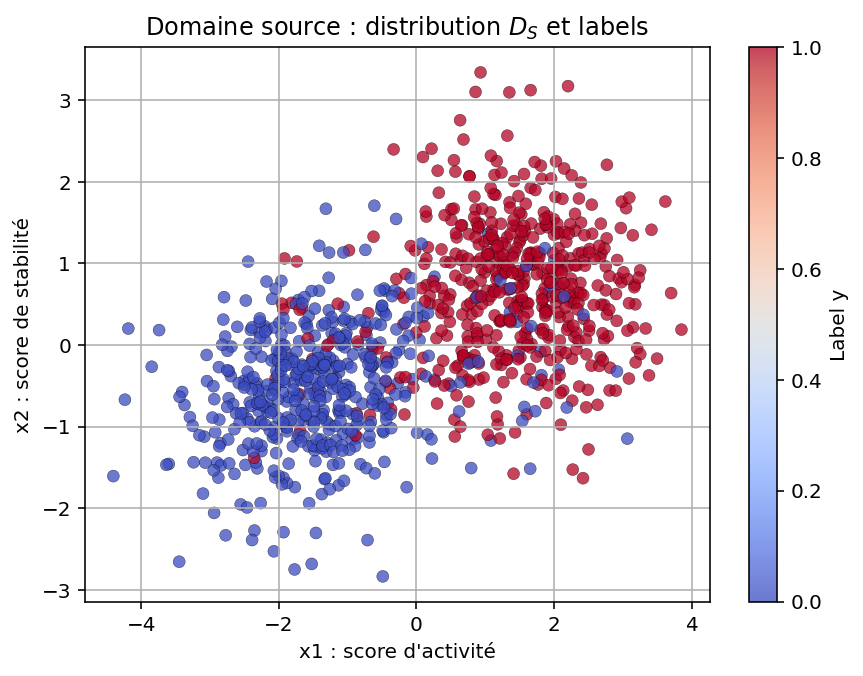
\includegraphics[width=0.8\textwidth]{Figure1.png}
    \caption{Distribution source et labels observés.}
\end{figure}


\end{frame}


\begin{frame}{Domaine cible \texorpdfstring{$\mathcal D_T=(D_T,f_T)$}{DT}}

\begin{figure}
    \centering
    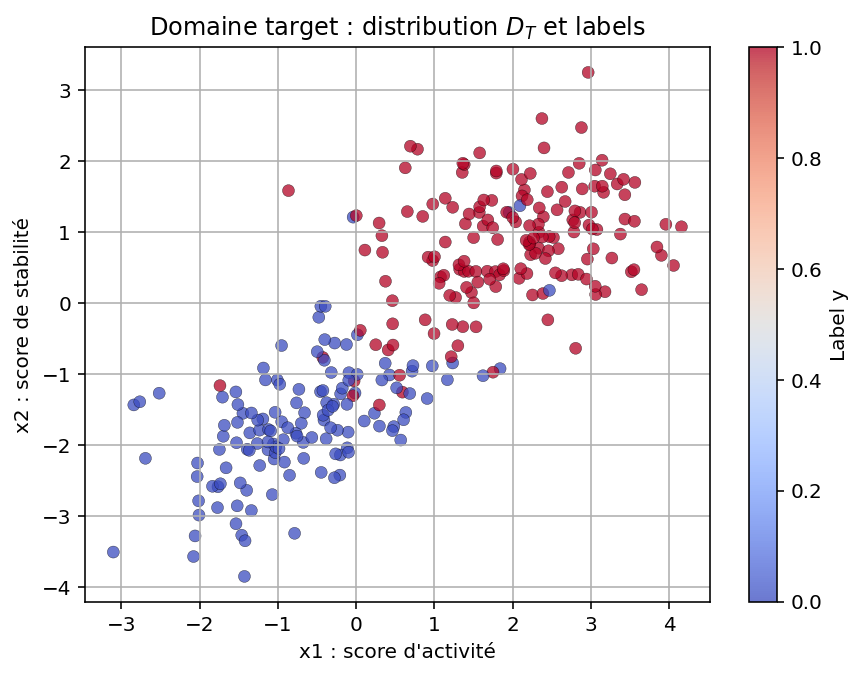
\includegraphics[width=0.8\textwidth]{Figure2.png}
\end{figure}

\end{frame}




\begin{frame}{Visualisation du décalage de domaine}

\begin{figure}
    \centering
    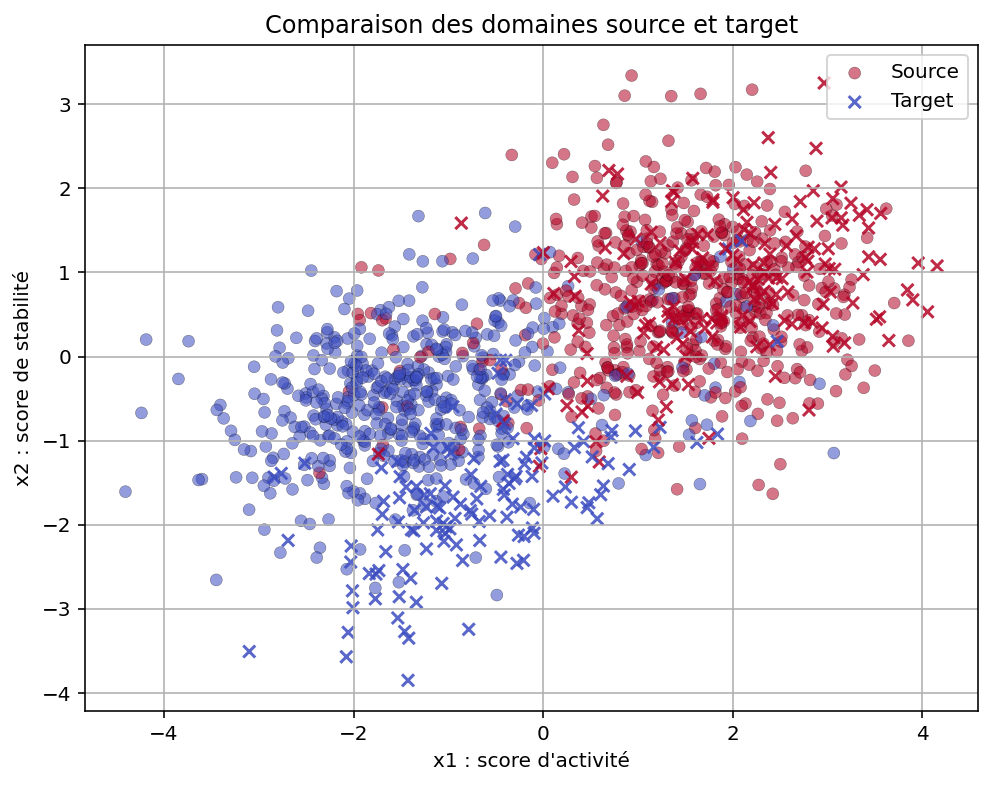
\includegraphics[width=0.70\textwidth]{Figure3.png}
\end{figure}
\[
D_S \neq D_T
\qquad \Longrightarrow \qquad
d_{\mathcal H\Delta\mathcal H}(D_S,D_T)>0.
\]

\end{frame}




\begin{frame}{Interprétation du Théorème 2}

\[
\varepsilon_T(h)
\le
\varepsilon_S(h)
+\frac12 d_{\mathcal H\Delta\mathcal H}(D_S,D_T)
+\lambda.
\]

\begin{itemize}
    \item \(\varepsilon_S(h)\) : erreur sur le domaine source ;
    \item \(d_{\mathcal H\Delta\mathcal H}\) : divergence entre les distributions ;
    \item \(\lambda\) : compatibilité des tâches source et cible.
\end{itemize}

Dans notre exemple :
\[
\varepsilon_S(h)\ \text{faible},\qquad
d_{\mathcal H\Delta\mathcal H}\ \text{modéré},\qquad
\lambda\ \text{faible}.
\]

\end{frame}




\end{document}